\documentclass[12pt]{article}
\usepackage[margin=0.75in]{geometry}
\usepackage{float}
\usepackage{multicol}
\usepackage{lmodern}
\usepackage{amssymb,amsmath}
\usepackage{ifxetex,ifluatex}
\usepackage{fixltx2e} % provides \textsubscript
\ifnum 0\ifxetex 1\fi\ifluatex 1\fi=0 % if pdftex
  \usepackage[T1]{fontenc}
  \usepackage[utf8]{inputenc}
\else % if luatex or xelatex
  \ifxetex
    \usepackage{mathspec}
    \usepackage{xltxtra,xunicode}
  \else
    \usepackage{fontspec}
  \fi
  \defaultfontfeatures{Mapping=tex-text,Scale=MatchLowercase}
  \newcommand{\euro}{€}
\fi
% use upquote if available, for straight quotes in verbatim environments
\IfFileExists{upquote.sty}{\usepackage{upquote}}{}
% use microtype if available
\IfFileExists{microtype.sty}{%
\usepackage{microtype}
\UseMicrotypeSet[protrusion]{basicmath} % disable protrusion for tt fonts
}{}
\usepackage{longtable,booktabs}
\usepackage{graphicx}
\makeatletter
\def\maxwidth{\ifdim\Gin@nat@width>\linewidth\linewidth\else\Gin@nat@width\fi}
\def\maxheight{\ifdim\Gin@nat@height>\textheight\textheight\else\Gin@nat@height\fi}
\makeatother
% Scale images if necessary, so that they will not overflow the page
% margins by default, and it is still possible to overwrite the defaults
% using explicit options in \includegraphics[width=3.5in][width, height, ...]{}
\setkeys{Gin}{width=\maxwidth,height=\maxheight,keepaspectratio}
\ifxetex
  \usepackage[setpagesize=false, % page size defined by xetex
              unicode=false, % unicode breaks when used with xetex
              xetex]{hyperref}
\else
  \usepackage[unicode=true]{hyperref}
\fi
\hypersetup{breaklinks=true,
            bookmarks=true,
            pdfauthor={Brandon LeBeau},
            pdftitle={PSQF 4143: Section 5},
            colorlinks=true,
            citecolor=blue,
            urlcolor=blue,
            linkcolor=magenta,
            pdfborder={0 0 0}}
\urlstyle{same}  % don't use monospace font for urls
\setlength{\parindent}{0pt}
\setlength{\parskip}{6pt plus 2pt minus 1pt}
\setlength{\emergencystretch}{3em}  % prevent overfull lines
\setcounter{secnumdepth}{0}

\title{PSQF 4143: Section 5}
\author{Brandon LeBeau}
\date{}

\begin{document}
\maketitle

\section{Tester}\label{tester}

\begin{itemize}
\itemsep1pt\parskip0pt\parsep0pt
\item
  For the score distribution below, which of the following score changes
  yields the greatest change in percentile rank?

  \begin{itemize}
  \itemsep1pt\parskip0pt\parsep0pt
  \item
    70 to 80
  \item
    80 to 90
  \item
    90 to 100
  \item
    The change is equal
  \item
    Cannot determine
  \end{itemize}
\end{itemize}

\begin{figure}[H]
\centering
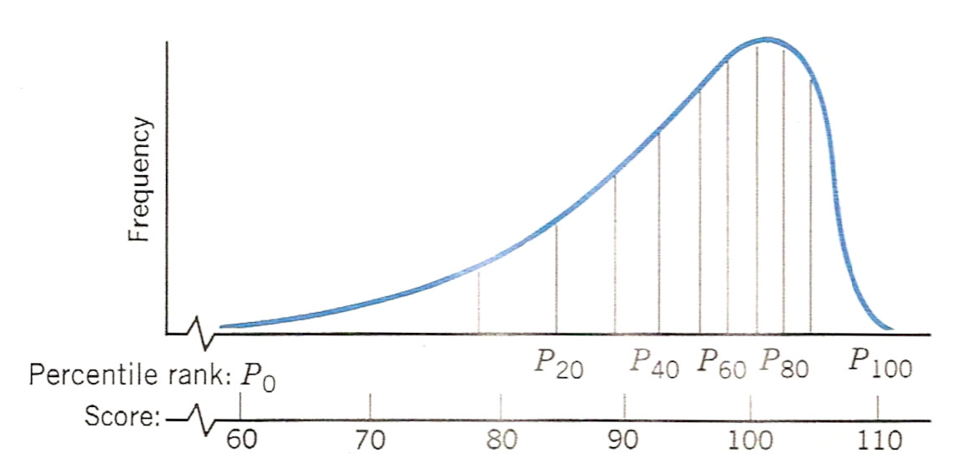
\includegraphics[width=3.5in]{pr_ques.png}
\caption{Dist}
\end{figure}

\section{Motivating Example}\label{motivating-example}

\begin{longtable}[c]{@{}lccc@{}}
\toprule
& Univ 1 & Univ 2 & Univ 3\tabularnewline
\midrule
\endhead
Score & 60 & 60 & 60\tabularnewline
Mean & 70 & 50 & 55\tabularnewline
SD & 10 & 20 & 2.5\tabularnewline
\bottomrule
\end{longtable}

\begin{itemize}
\itemsep1pt\parskip0pt\parsep0pt
\item
  Which score is more extreme?
\item
  We can transform into \emph{Standard Scores}.
\end{itemize}

\section{Linear Transformations}\label{linear-transformations}

\begin{itemize}
\itemsep1pt\parskip0pt\parsep0pt
\item
  A linear transformation is an algebraic rule for changing scores in a
  distribution where the distance between scores are preserved.

  \begin{itemize}
  \itemsep1pt\parskip0pt\parsep0pt
  \item
    This means the shape of the distribution is unchanged.
  \end{itemize}
\item
  Example:

  \begin{itemize}
  \itemsep1pt\parskip0pt\parsep0pt
  \item
    Suppose we want to change scores by multiplying each score by 5 and
    adding 20
  \item
    Let X be the original score
  \item
    Then \(Y = X*5 + 20\)
  \item
    Y is then said to be a linear transformation of X
  \end{itemize}
\end{itemize}

\section{Linear Transformation
Example}\label{linear-transformation-example}

\begin{itemize}
\itemsep1pt\parskip0pt\parsep0pt
\item
  Suppose we have the following scores:

  \begin{itemize}
  \itemsep1pt\parskip0pt\parsep0pt
  \item
    X: 3, 5, 7, 9, 11
  \item
    Y: 35, 45, 55, 65, 75
  \end{itemize}
\end{itemize}

\begin{figure}[H]
\centering
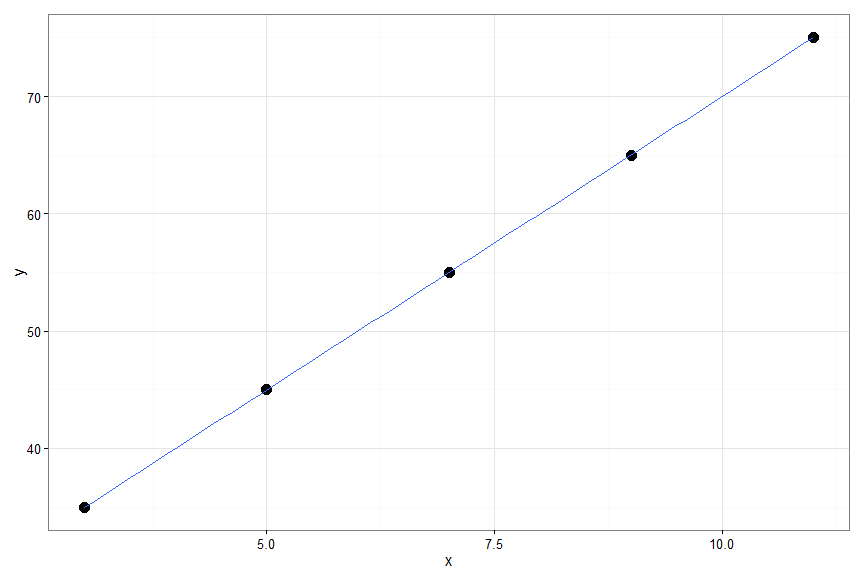
\includegraphics[width=3.5in]{figure/ltplot-1.png}
\caption{plot of chunk ltplot}
\end{figure}

\section{Linear Transformations
(cont.)}\label{linear-transformations-cont.}

\begin{itemize}
\itemsep1pt\parskip0pt\parsep0pt
\item
  In general we can multiply by any value and add any value:

  \begin{itemize}
  \itemsep1pt\parskip0pt\parsep0pt
  \item
    \(Y = bX + a\)
  \item
    Where Y is transformed scores
  \item
    X is the original scores
  \item
    b is the multiplicative constant
  \item
    a is the additive constant
  \end{itemize}
\end{itemize}

\section{Add a constant to every
score}\label{add-a-constant-to-every-score}

\[Y = X + a\] \[b = 1\] - a must be a real number

\begin{figure}[H]
\centering
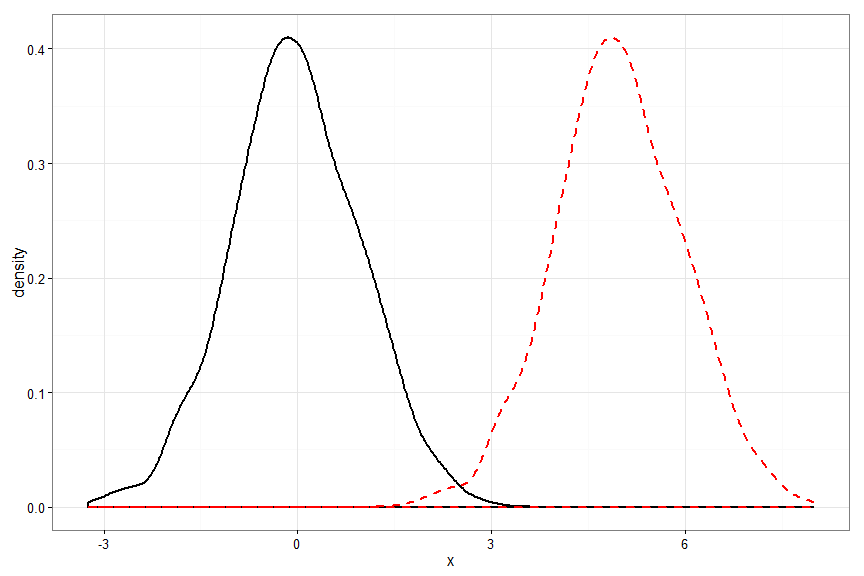
\includegraphics[width=3.5in]{figure/addconstant-1.png}
\caption{plot of chunk addconstant}
\end{figure}

\section{Add a constant: Data
Example}\label{add-a-constant-data-example}

\begin{longtable}[c]{@{}lccc@{}}
\toprule
& X & \(Y = X + 2\) & \(Y = X - 4\)\tabularnewline
\midrule
\endhead
& 4 & 6 & 0\tabularnewline
& 5 & 7 & 1\tabularnewline
& 6 & 8 & 2\tabularnewline
& 7 & 9 & 3\tabularnewline
& 8 & 10 & 4\tabularnewline
\midrule 
Sum X & 30 & 40 & 10\tabularnewline
Sum \(X^2\) & 190 & 330 & 30\tabularnewline
mean & 6 & 8 & 2\tabularnewline
var & 2 & 2 & 2\tabularnewline
std dev & 1.4 & 1.4 & 1.4\tabularnewline
\bottomrule
\end{longtable}

\begin{itemize}
\itemsep1pt\parskip0pt\parsep0pt
\item
  Rule 1:

  \begin{itemize}
  \itemsep1pt\parskip0pt\parsep0pt
  \item
    If \(Y = X + a\)
  \item
    Then \(\bar{Y} = \bar{X} + a\)
  \end{itemize}
\item
  Rule 2:

  \begin{itemize}
  \itemsep1pt\parskip0pt\parsep0pt
  \item
    If \(Y = X + a\)
  \item
    Then \(s_{y}^2 = s_{x}^2\)
  \item
    and \(s_{y} = s_{x}\)
  \end{itemize}
\end{itemize}

\section{Multiply every score by a
constant}\label{multiply-every-score-by-a-constant}

\[Y = bX\] \[a = 0\] - b must be a real number

\begin{figure}[H]
\centering
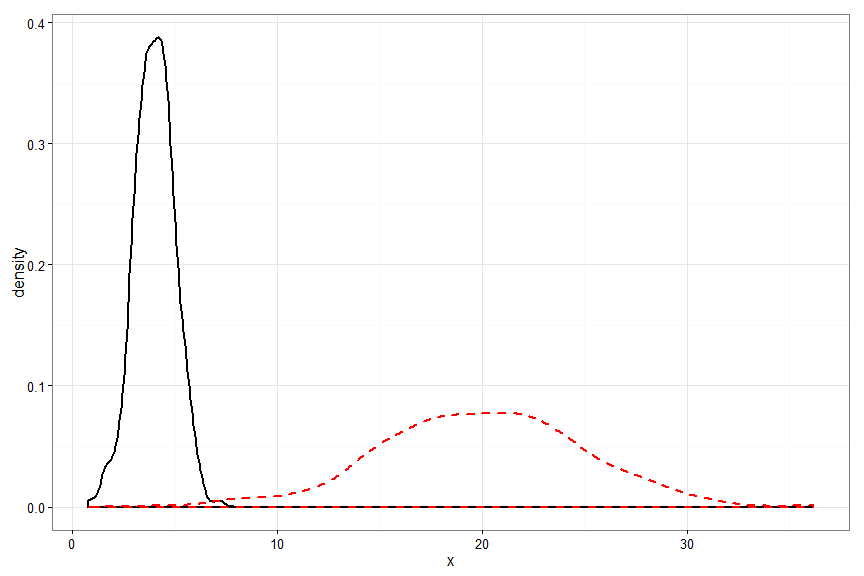
\includegraphics[width=3.5in]{figure/multiplyconstant-1.png}
\caption{plot of chunk multiplyconstant}
\end{figure}

\section{Multiply a constant: Data
Example}\label{multiply-a-constant-data-example}

\begin{longtable}[c]{@{}lccc@{}}
\toprule
& X & \(Y = 2X\) & \(Y = -4X\)\tabularnewline
\midrule
\endhead
& 4 & 8 & -16\tabularnewline
& 5 & 10 & -20\tabularnewline
& 6 & 12 & -24\tabularnewline
& 7 & 14 & -28\tabularnewline
& 8 & 16 & -32\tabularnewline
\midrule
Sum X & 30 & 60 & -120\tabularnewline
Sum \(X^2\) & 190 & 760 & 3040\tabularnewline
mean & 6 & 12 & -24\tabularnewline
var & 2 & 8 & 32\tabularnewline
std dev & 1.4 & 2.8 & 5.6\tabularnewline
\bottomrule
\end{longtable}

\begin{itemize}
\itemsep1pt\parskip0pt\parsep0pt
\item
  Rule 1:

  \begin{itemize}
  \itemsep1pt\parskip0pt\parsep0pt
  \item
    If \(Y = bX\)
  \item
    Then \(\bar{Y} = \bar{X} * b\)
  \end{itemize}
\item
  Rule 2:

  \begin{itemize}
  \itemsep1pt\parskip0pt\parsep0pt
  \item
    If \(Y = X + a\)
  \item
    Then \(s_{y}^2 = b^2s_{x}^2\)
  \item
    and \(s_{y} = |b|s_{x}\)
  \end{itemize}
\end{itemize}

\section{Multiply by a constant, then add a
constant}\label{multiply-by-a-constant-then-add-a-constant}

\[Y = bX + a\] - a and b must be real numbers

\begin{figure}[H]
\centering
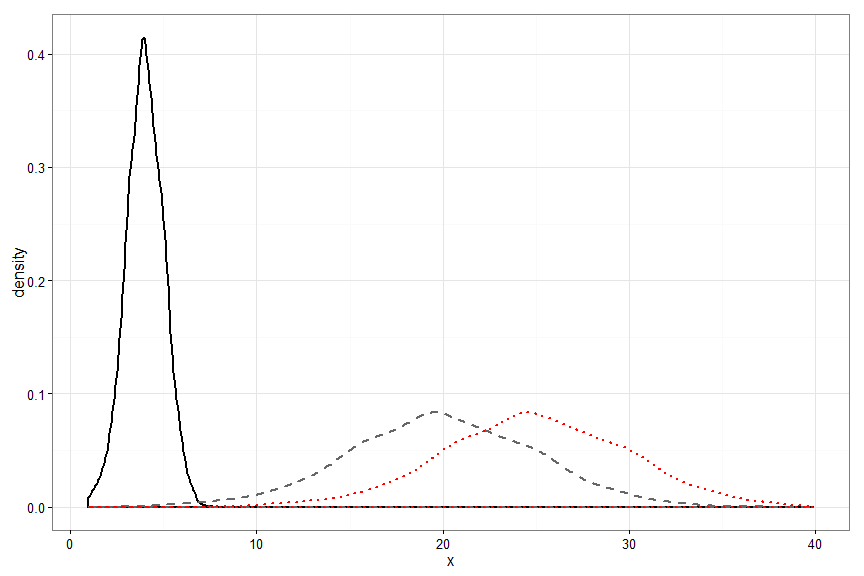
\includegraphics[width=3.5in]{figure/multaddconstant-1.png}
\caption{plot of chunk multaddconstant}
\end{figure}

\section{Multiply a constant, add constant: Data
Example}\label{multiply-a-constant-add-constant-data-example}

\begin{longtable}[c]{@{}lcc@{}}
\toprule
& X & \(Y = 2X - 2\)\tabularnewline
\midrule
\endhead
& 4 & 6\tabularnewline
& 5 & 8\tabularnewline
& 6 & 10\tabularnewline
& 7 & 12\tabularnewline
& 8 & 14\tabularnewline
\midrule
Sum X & 30 & 50\tabularnewline
Sum \(X^2\) & 190 & 540\tabularnewline
mean & 6 & 10\tabularnewline
var & 2 & 8\tabularnewline
std dev & 1.4 & 2.8\tabularnewline
\bottomrule
\end{longtable}

\begin{itemize}
\itemsep1pt\parskip0pt\parsep0pt
\item
  Rule 1:

  \begin{itemize}
  \itemsep1pt\parskip0pt\parsep0pt
  \item
    If \(Y = bX + a\)
  \item
    Then \(\bar{Y} = \bar{X} * b + a\)
  \item
    and \(s_{y}^2 = b^2s_{x}^2\)
  \item
    and \(s_{y} = |b|s_{x}\)
  \end{itemize}
\end{itemize}

\section{Example}\label{example}

\begin{itemize}
\itemsep1pt\parskip0pt\parsep0pt
\item
  Suppose the mean score on an attitude survey was 23 and the SD was 7.
  The score distribution was transformed by \(Y = 3X + 11\).

  \begin{itemize}
  \itemsep1pt\parskip0pt\parsep0pt
  \item
    What is the mean of the transformed scores?
  \item
    What is the SD of the transformed scores?
  \end{itemize}
\end{itemize}

\section{Special Linear
Transformation}\label{special-linear-transformation}

\begin{itemize}
\itemsep1pt\parskip0pt\parsep0pt
\item
  One transformation has been used a lot and has a special name called
  \emph{Standard Scores}, \emph{Normal Scores}, or more commonly
  \emph{z-scores}.
\end{itemize}

\[Y = \frac{1}{s_{x}}X + \frac{-\bar{X}}{s_{x}}\]

\begin{itemize}
\item
  where \(b = \frac{1}{s_{s}}\) and \(a = \frac{-\bar{X}}{s_{x}}\)
\item
  This can be reformulated as:
\end{itemize}

\[Z = \frac{(X - \bar{X})}{s_{x}}\]

\section{z-score examples}\label{z-score-examples}

\begin{itemize}
\itemsep1pt\parskip0pt\parsep0pt
\item
  What z-score corresponds to a raw score of 60 in a distribution having
  a mean of 70 and a standard deviation of 20?
\item
  In a distribution with a mean of 23 and a standard deviation of 4,
  what raw score corresponds to a z-score of -2.25?
\end{itemize}

\section{z-score properties}\label{z-score-properties}

\[\bar{z} = 0\] \[s_{z} = 1\] \[s_{z}^2 = 1\]

\begin{itemize}
\item
  z-scores are great for comparing distributions that have different
  means and standard deviations.
\item
  To backtransform z-scores: \[X = s_{x} * z + \bar{X}\]
\end{itemize}

\section{Transform z-score example}\label{transform-z-score-example}

\begin{itemize}
\item
  In a distribution with a mean of 71 and a SD of 18, a raw score of 85
  was found. What is the equivalent score in a distribution with a mean
  of 50 and a standard deviation of 10?
\item
  More formally:
  \[ X_{n} = \left(\frac{s_{n}}{s_{o}} \right) X_{o} + \bar{X}_{n} - \left(\frac{s_{n}}{s_{o}} \right) \bar{X}_{o} \]
\end{itemize}

\section{Other common scales}\label{other-common-scales}

\begin{itemize}
\itemsep1pt\parskip0pt\parsep0pt
\item
  z-scores are also useful to place scores on a desired scale.
\item
  There are many common scales that have been used over time.

  \begin{itemize}
  \itemsep1pt\parskip0pt\parsep0pt
  \item
    T-scores: mean of 50, sd of 10
  \item
    Stanines: mean of 5, sd of 2
  \item
    Normal Curve Equivalents (NCE): mean of 50, sd of 21
  \item
    SAT: mean of 500, sd of 100, rounded to nearest 10
  \item
    ACT: mean of 21, sd of 5, rounded to nearest whole number
  \item
    GRE: mean of 150, sd of 8.75
  \end{itemize}
\end{itemize}

\begin{figure}[H]
\centering
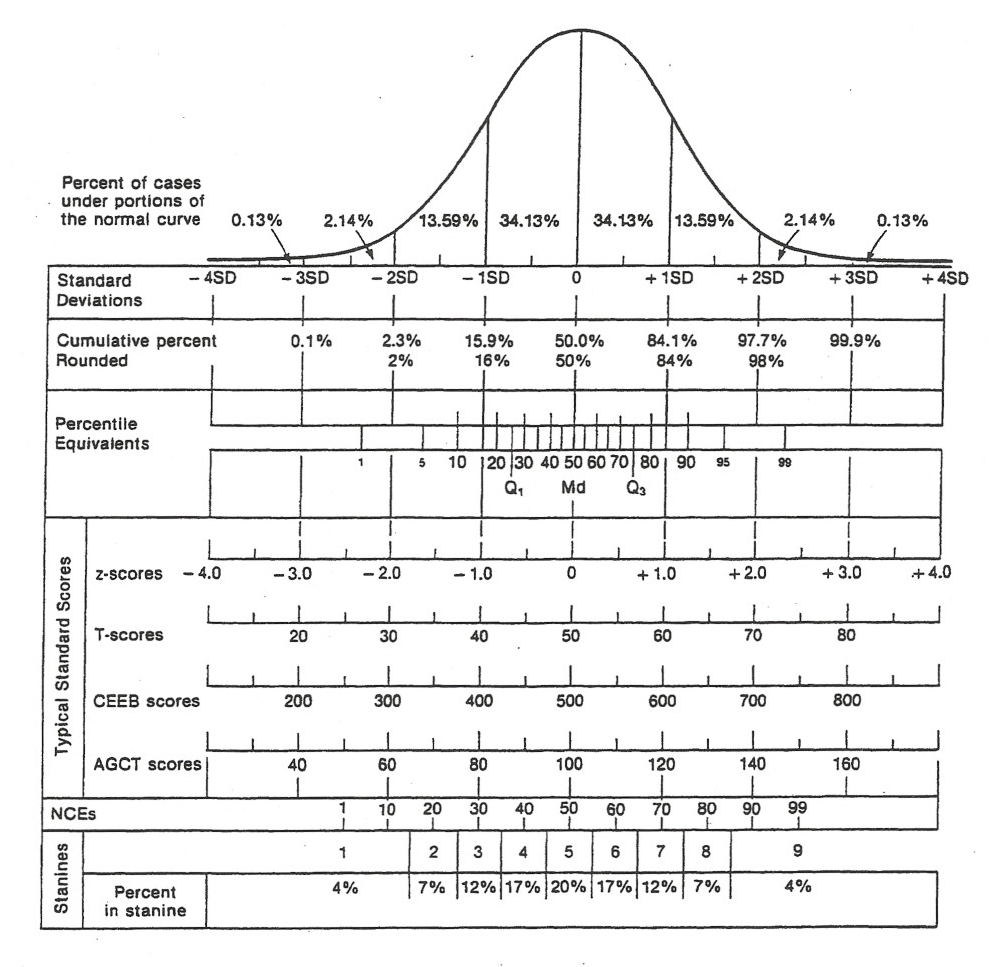
\includegraphics[width=3.5in]{standardscores.png}
\caption{Score Scales}
\end{figure}

\section{Combining scores from different
scales}\label{combining-scores-from-different-scales}

\begin{itemize}
\itemsep1pt\parskip0pt\parsep0pt
\item
  Suppose two students are competing for a college scholarship, and we
  need to decide which student has a better academic record.
\end{itemize}

\begin{longtable}[c]{@{}lccc@{}}
\toprule
& ACT & HSGPA & Total\tabularnewline
\midrule
\endhead
A & 25 & 3.7 & 28.7\tabularnewline
B & 31 & 3.3 & 34.3\tabularnewline
\midrule
Mean & 28 & 3.5 &\tabularnewline
SD & 3 & 0.2 &\tabularnewline
\bottomrule
\end{longtable}

\section{Normalizing Transformations}\label{normalizing-transformations}

\begin{itemize}
\itemsep1pt\parskip0pt\parsep0pt
\item
  Linear transformations preserve the shape of the distribution.
\item
  This is one of their strengths and why they are used extensively.
\item
  However, as we progress to inferential statistics, our methods assume
  a normal distribution or bell curve.
\item
  As such, what to do with skewed distributions?
\item
  There are nonlinear transformations that can take a skewed
  distribution and transform it to behave more normal.

  \begin{itemize}
  \itemsep1pt\parskip0pt\parsep0pt
  \item
    These transformations change the shape and thus the distance between
    scores.
  \end{itemize}
\end{itemize}

\begin{figure}[H]
\centering
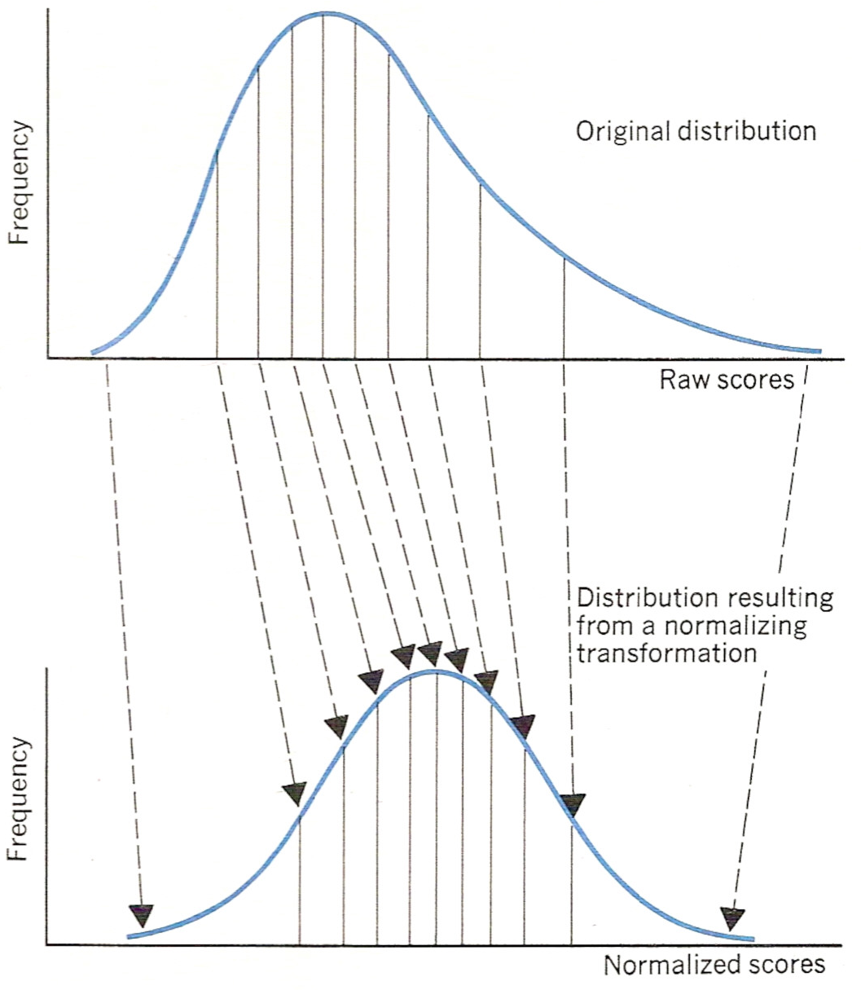
\includegraphics[width=3.5in]{normalizingtransformation.png}
\caption{Normalizing Transformation}
\end{figure}

\end{document}
